% ****** Start of file aipsamp.tex ******
%
%   This file is part of the AIP files in the AIP distribution for REVTeX 4.
%   Version 4.1 of REVTeX, October 2009
%
%   Copyright (c) 2009 American Institute of Physics.
%
%   See the AIP README file for restrictions and more information.
%
% TeX'ing this file requires that you have AMS-LaTeX 2.0 installed
% as well as the rest of the prerequisites for REVTeX 4.1
% 
% It also requires running BibTeX. The commands are as follows:
%
%  1)  latex  aipsamp
%  2)  bibtex aipsamp
%  3)  latex  aipsamp
%  4)  latex  aipsamp
%
% Use this file as a source of example code for your aip document.
% Use the file aiptemplate.tex as a template for your document.
\documentclass[%
 aip,
% jmp,
% bmf,
% sd,
% rsi,
 amsmath,amssymb,
%preprint,%
 reprint,%
%author-year,%
%author-numerical,%
% Conference Proceedings
]{revtex4-1}

\usepackage{graphicx}% Include figure files
%\usepackage{dcolumn}% Align table columns on decimal point

%\usepackage[mathlines]{lineno}% Enable numbering of text and display math
%\linenumbers\relax % Commence numbering lines
\usepackage[utf8]{inputenc}
\usepackage[T1]{fontenc}
\usepackage{mathptmx}
\usepackage{lipsum}
\usepackage{amsmath}
\usepackage{physics}
\usepackage{xparse}
\usepackage{bbm}
\usepackage{hyperref}
%\usepackage{multirow}
%\usepackage{makecell}
\graphicspath{{Pictures/}}

\renewcommand*{\figureautorefname}{Fig.}

\newcommand{\mytitile}{Effects of intense light-matter interaction in a superconducting artificial molecule}
\begin{document}
	\preprint{AIP/123-QED}
	
	\title[\mytitile]{\mytitile\\~}
	
	\author{G.P. Fedorov}
	\email{gleb.fedorov@phystech.edu}
	
	\affiliation{ 
		Russian Quantum Center, Skolkovo village, Russia
	}%
	\affiliation{ 
		Moscow Institute of Physics and Technology, Dolgoprundiy, Russia
	}%
	
	\author{V.B. Yursa}
	\affiliation{ 
		Moscow Institute of Physics and Technology, Dolgoprundiy, Russia
	}%
	
	\author{A. Efimov}
	
	\affiliation{ 
		Moscow Institute of Physics and Technology, Dolgoprundiy, Russia
	}%

	\author{K. Shiyanov}

	\affiliation{ 
		Moscow Institute of Physics and Technology, Dolgoprundiy, Russia
	}%

	\author{O.V. Astafiev}
	\affiliation{ 
		Moscow Institute of Physics and Technology, Dolgoprundiy, Russia 
	}%
	
	
	\date{\today}% It is always \today, today,
	%  but any date may be explicitly specified
	
	
	\begin{abstract}
		To build a full-scale quantum processor it is necessary to automate as many steps as possible on the physical, hardware level. Circuit quantum electrodynamics (cQED) is a contemporary architecture for dispersive readout and Purcell protection of superconducting qubits of various types, and thus it is necessary to develop software that is able to perform every kind of automatic calibration of such systems from scratch without any human participation. An important step towards this goal is to build a noise-insensitive and accurate computer vision tool to process three-dimensional spectroscopic data. In this work, we present and describe two scalable algorithms that are able to extract the Hamiltonian parameters of the cQED systems from spectroscopic data. 
	\end{abstract}
	
	\maketitle
\section{Introduction}
Over the past twenty years, many 


A sufficiently large anharmonicity is needed to prevent qubit operations from exciting other transitions in the system. Therefore, we will use two- and three-level approximations for our calculations


A quantum system exposed to external driving, can experience a number of quantum phenomena due to the resonant transitions between energy levels. The most known examples are coherent population trapping, electromagnetically induced transparency (EIT)\cite{boller1991observation}, stimulated Raman adiabatic passage\cite{bergmann1998coherent} and Autler-Townes (AT) splitting\cite{autler1955stark} which can happen in systems with just three energy levels. 
The main attention in our work is paid to the last effect, which related to the dressed states.
The AT effect has been studied in atomic\cite{picque1976direct} and molecular systems\cite{tamarat1995pump}, quantum dots\cite{xu2007coherent}, and superconducting qubits\cite{li2011decoherence, novikov2013autler}.

If the driving field is strong the interaction between the system and the field become significant and leads to oscillates with Rabi frequency. The new energy state called dressed states. If an additional weak probing field is applied, the spectra of the strongly driven system can be probed. In particular the dressed state model nicely explains the emergence of the Mollow triplet\cite{newstein1968spontaneous} spectrum, which consists of a central peak with two side bands separated by the Rabi frequency.

For example, the implementation of the controlled-PHASE quantum gate for typical alkali atoms (such as Rb or Cs)  is based on the effect of dressed states in conjunction with the effect of Rydberg-blockade\cite{sun2018analysis}. One of the possible way to build quantum memory with trapped atomic ions based on dressed states is described in this work\cite{timoney2011quantum}. 

In this article will be shown how the spectrum of the system depends on drivers on different qubits and explicitly shown the dressed states.%\autoref{sec:level1}
 
\section{Methods}
\subsection{Theoretical description of the system}

We investigate a system of two interacting transmons. The transmon\cite{koch2007charge} represents two Josephson junctions (dc-SQUID) which are shunted by an additional large capacitance(compared to other capacitances in the circuit). This dc-SQUID setup allows for the tuning of the Josephson energy $E_J = E_J^{max}|\cos(\pi \frac{\Phi}{\Phi_0})|$  by
means of an external magnetic flux $\Phi$. The transmon can be considered as an oscillator with a quartic perturbation describing the leading-order anharmonicity. The system of two transmons and their connection forms a level system.

In this section we analyse theoretically two qubit system.
 In our study we used transmons.The transmon Hamiltonian is $H = 4\cdot E_C(n-n_g)^2 -E_J\cos(\phi)$, where $E_c $ and $E_J$ -charge and Josephson energy respectively. The symbols $n$ and $\phi$ denote the number of Cooper pairs transferred between the islands and the
 gauge-invariant phase difference between the superconductors,
 respectively.
 When the ratio $\frac{E_C}{E_J}$ is large the perturbation approach can
 be employed. After the expansion of the cosine for small angles and neglecting of the small terms the Hamiltonian can be
 viewed as a harmonic oscillator with a quartic perturbation describing the leading-order anharmonicity.
 After conversion to dimensionless variables and neglecting small terms and set $\hbar = 1$, we move to the new Hamiltonian of transmon. 
\begin{equation}
H_{tr}= \omega_{tr} b^{\dagger}b +\frac{1}{2}\alpha b^{\dagger}b(b^{\dagger}b-1)
\end{equation}
Where $\alpha=-E_C$, $\omega_{tr}=\sqrt{8E_CE_J}+\alpha$.


The implementations of the transitions between the eigenstates is achieved by external microwave driving through a capacitively coupled transition line. In the notations used above, the pump Hamiltonian can be written generically as $ 	H_{dr} = -2e n\beta V_{dr}(t)=\Omega(t)(b+b^{\dagger})$.
Where $2en$ -- the charge on island, $\beta$ -- dimensionless coefficient depending on the geometry of the system and the ratio of capacities, $V_{dr}(t)$ -- the voltage on the external source.

For simplifications select the dependence on time:
\begin{equation}
H_{dr} = \Omega\cos(\omega_d t)(b+b^{\dagger})
\end{equation}
Let's move on to the consideration of the two-qubit system. The complete Hamiltonian will contain the members responsible for transmons, the drives on each of them separately with frequencies $\omega_d$ and $\omega_d+\delta_{\omega}$ respectively, and the interaction term between qubits:
\begin{equation}\label{Hsystem}
H_{system}= H_{tr1}+H_{tr2}+H_{dr1}+H_{dr2}+H_{int}
\end{equation}
Where $H_{int}= J(bc^{\dagger}+b^{\dagger}c)$, $b^{\dagger}$;$b$ and $c^{\dagger}$,$c$ - denote the regular annihilation and creation operators
for the harmonic oscillator approximating both of qubits respectively.



\begin{figure*}
	\centering
	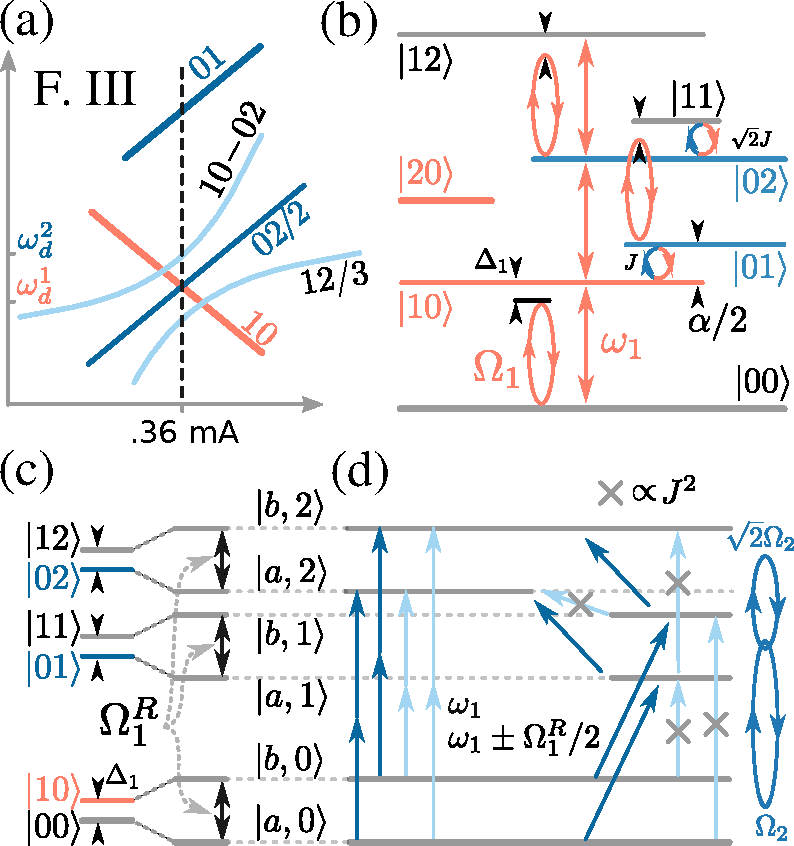
\includegraphics[width=.9\linewidth]{main_scheme}
	\caption{Explaining the origin of the AT satellites. \textbf{(a)} System level structure at 3.65 mA. At this current, the first transmon (orange) is below the second one (blue) exactly by $\alpha/2$ ($\omega_2 - \omega_1 = \alpha/2$), and thus $E_{02} - E_{10} = \hbar\omega_1$. Since $E_{12} - E_{02} = \omega_1$ as well, both $00\rightarrow 10$, two-photon $00 \rightarrow 02/2$ and three-photon $00\rightarrow 12/3$ transitions can occur around the same frequency of $\omega_1$. During the two-tone spectroscopy, the first transmon is driven by a strong signal of amplitude $\Omega_1$ (possibly, at a small detuning $\Delta_1$ from $\omega_1$ shown in green). The transmon-transmon interaction in RWA conserves the number of excitations and is depicted as orange-blue circles. \textbf{(b)} Moving to the frame rotating with the drive of the first transmon, we make all the states $\ket{0j},\ket{1j}$ nearly degenerate (in fact, now the first transmon splitting equals $\Delta_1$). However, the presence of a strong excitation lifts the degeneracy and the splitting changes to $\Omega_1^R = \sqrt{\Omega_1^2 + \Delta_1^2}$ (the first transmon becomes light-dressed). \textbf{(c)} Transitions in the light-dressed system when the second qubit is excited (level subspaces coupled by the corresponding drive operator are shown as blue ellipses). In the left part of the panel, all possible two-photon transitions near $\omega_1$ are depicted. The structure of the levels gives rise to three cases: the green transitions are not shifted in frequency, the orange are red-shifted by $\Omega_R^1/2$ and the blue are blue-shifted by $\Omega_R^2/2$. However, as shown in the right part of the panel, without the transmon-transmon interaction the satellite transitions are forbidden due the selection rule: $\bra{a,j}\hat{\mathbbm{1}}\otimes \hat n_2 \ket{b, j+1} = 0$ since $\braket{a}{b} = 0$. When the coupling equals $J$, the dispersive approximation yields $\bra{a,j}\hat{\mathbbm{1}}\otimes \hat n_2\ket{b, j+1}\propto J^2/(\omega_1-\omega_2)^2$ and the satellites become visible. Remarkably, due to the two-photon nature of the transitions, the Autler-Townes splitting in this case will be two $\Omega_1^R$.}
	\label{fig:main_scheme}
\end{figure*}



\subsection{Master equation solution in QuTip}

\subsection{Experiment}
\subsubsection{Device design and fabrication}
The chip consist the transmission line capacitively couple to $\lambda/4$ coplanar waveguide resonator which capacitively couple to two transmons. Qubit control is achieved by external microwave driving line and two flux bias lines. 
\subsubsection{Experimental parameters}
\subsubsection{Experimental setup}
The sample was measured in laboratory of artificial quantum systems at Moscow Institute of Physics and Technology. Cryogenic equipment was
represented by BlueFors LD250 dilution refrigerator, with base temperature of 16 mK. The microwave equipment included KEYSIGHT PNA-L N5232A 300 kHz-20 GHz vector network analyser, Agilent MXG N5183B 9 kHz - 40 GHz analog signal generator. The sample was 
flux biased using YOKOGAWA GS200 current source.

Microwave line was thermalized with 60 dB of attenuation, additional 20 dB of attenuation were introduced on a directional coupler which added the second tone from the $\mu$-wave source. After leaving the sample the signal passed through two isolators and a hybrid coupler. Finally, the signal was amplified with 4-8 GHz LNF amplifier at 4 K and a with a room-temperature amplifier.

\section{Results}
\subsection{\label{sec:level1} Experimental and numerical parts}
Two tone spectroscopy was found experimentally and shows good agreement with modelling data\autoref{fig:two-tone}. 

\begin{figure*}
	\centering
	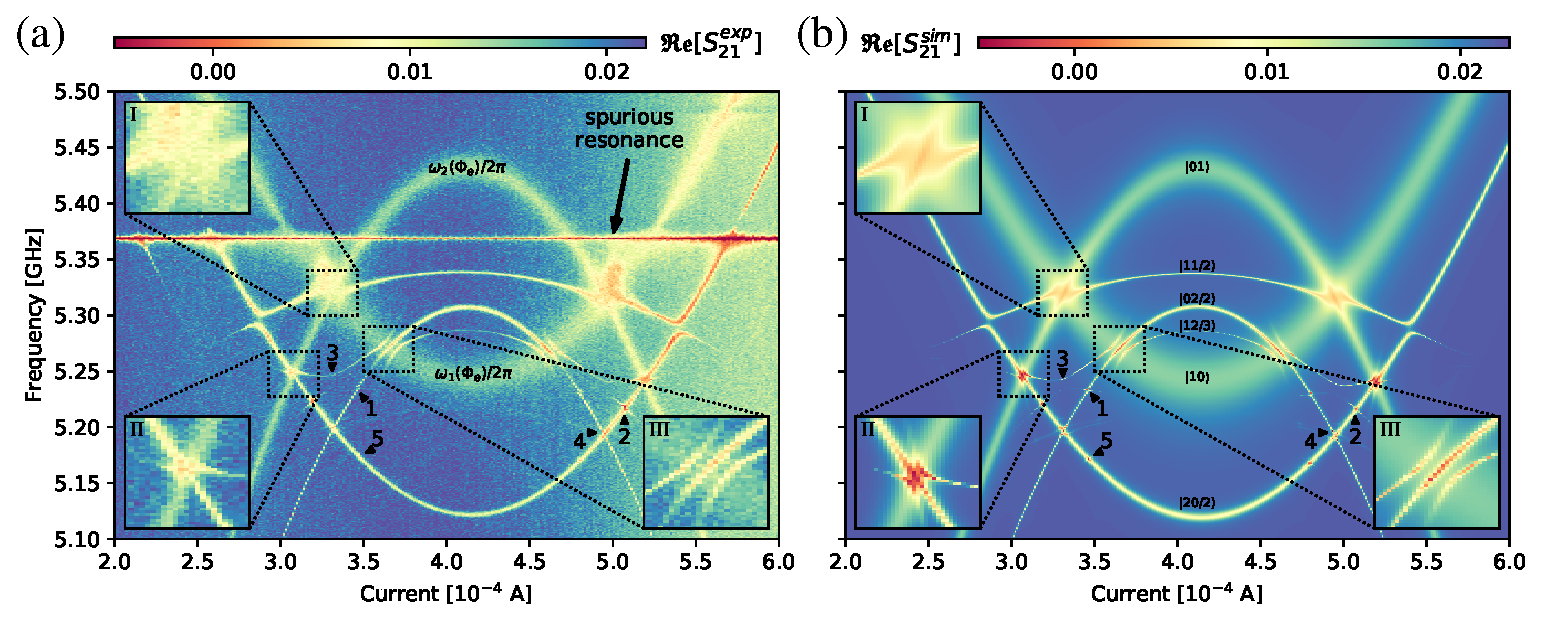
\includegraphics[width=\linewidth]{main_picture}
	\caption{Two-tone spectroscopy: \textbf{(a)} Experiment;\textbf{(b)} Modelling ; the colorbar is common.  Clear flux-dependent transmon transitions are visible.}
	\label{fig:two-tone}
\end{figure*}

We obtain illustrative example of dressed states\autoref{fig:difdrive}. On this figure the microwave drive acts only on the one of qubits. 
\begin{figure}[h]
	\centering
	\includegraphics[width=\linewidth]{drawing}
	\caption{Drive acts on the one of qubit, with different amplitude 100,200,300 MHz}
	\label{fig:difdrive}
\end{figure}


\subsection{Theoretical description of AF}
Let's consider our system (\autoref{Hsystem}) in rotating frame. Moving to this frame is achieved by the rotation:
\begin{equation}
R = \exp(-i\omega_d t (b^{\dagger}b+c^{\dagger}c))
\end{equation}  
After this transformation the effective Hamiltonian can be found from equation:
\begin{equation}
H_{system}^R = R^{\dagger}H_{system}R-iR^{\dagger}\dot{R}
\end{equation}

From the simulation follows that a two-level approximation for first qubit and three-level approximation for second is sufficient to observe the effect we are interested in. The Hamiltonian in matrix form is given by the following expression:
\begin{widetext}
	\begin{equation}\label{matrix} 
	\text{$H^R$} = \left(\begin{matrix}
	0 & \text{$\Omega_1/2 $} & \text{$\Omega _2$} e^{i \text{$\delta_{\omega}$} t}/2 & 0 & 0 & 0 \\
	\text{$\Omega_1/2 $} & \text{$-\Delta_1 $} & J & \text{$\Omega_2$} e^{i \text{$\delta_{\omega}$} t}/2 & 0 & 0 \\
	\text{$\Omega_2$} e^{-i \text{$\delta_{\omega} $} t}/2 & J & -\text{$\Delta_2 $} &
	\text{$\Omega_1$/2} & \sqrt{2} \text{$\Omega_2$} e^{i \text{$\delta_{\omega}$} t}/2 & 0 \\
	0 & \text{$\Omega_2$} e^{-i \text{$\delta_{\omega} $} t}/2 & \text{$\Omega_1/2$} &
	\text{$-\Delta_2 -\Delta_1$} & \sqrt{2} J & \sqrt{2} \text{$\Omega_2$} e^{i \text{$\delta_{\omega}
			$} t}/2 \\
	0 & 0 & \sqrt{2} \text{$\Omega_2$} e^{-i \text{$\delta_{\omega}$} t}/2 & \sqrt{2} J &
	\text{$\alpha$}-2 \text{$\Delta_2$} & \text{$\Omega_1/2$} \\
	0 & 0 & 0 & \sqrt{2} \text{$\Omega_2$} e^{-i \text{$\delta_{\omega} $} t}/2 & \text{$\Omega_1/2
		$} & \text{$\alpha$}-2 \text{$\Delta_2$}- \text{$\Delta_1$} \\
	\end{matrix}\right)
	\end{equation}
\end{widetext}
Where $\Omega_1$, $\Omega_2$ - amplitudes of the drives, $\Delta_1 = \omega_d-\omega_{tr1}=0$,$\Delta_2 = \omega_d-\omega_{tr2}$.
Let's consider the Hamiltonian (\autoref{matrix}) in details. Divide it into three parts: time-dependent $(V_t)$, the part responsible for the interaction between the qubits $(V_J)$ and all the rest $(H_0)$.
\begin{equation}
	H^R=H_0+V_J+V_t
\end{equation}
The $\Omega_1\gg \Omega_2,\Delta_2\gg J$, so the driven field on the first qubit is strong and form the dressed states defined by the Hamiltonian $H_0$.
The Hamiltonian $H_0$ is station and we can find eigenvectors and eigenvalues. The drive on the second qubit is weak with very low intensity, so we can neglect any perturbation introduced by second drive on the position, width os the dressed states.
Firstly, we consider the system of non-interacting qubits $(J=0)$. In this case some transitions are prohibited and the splitting we are interested in is not observed. 
Therefore a non-zero interaction between qubits is necessary to observe AT effect.

After that according to the perturbation theory (with perturbation $V_J$) to $H_0$ we found the first-order corrections to the wave functions. We can use Fermi Golden Rule to find the probability of transition.
\appendix
\section{Theoretical description of two-photon process}





\section{Text}


In order to determine which transitions correspond to the lines, the stationary Schrödinger equation was solved \autoref{fig:spectr} in three-level approximation for both of qubits. With the Hamiltonian of the system:
\begin{equation}
	H_{system} = H_{tr1}\otimes\mathbbm{1}+\mathbbm{1}\otimes H_{tr2}+H_{int}
\end{equation}
\begin{figure}[h]
	\centering
	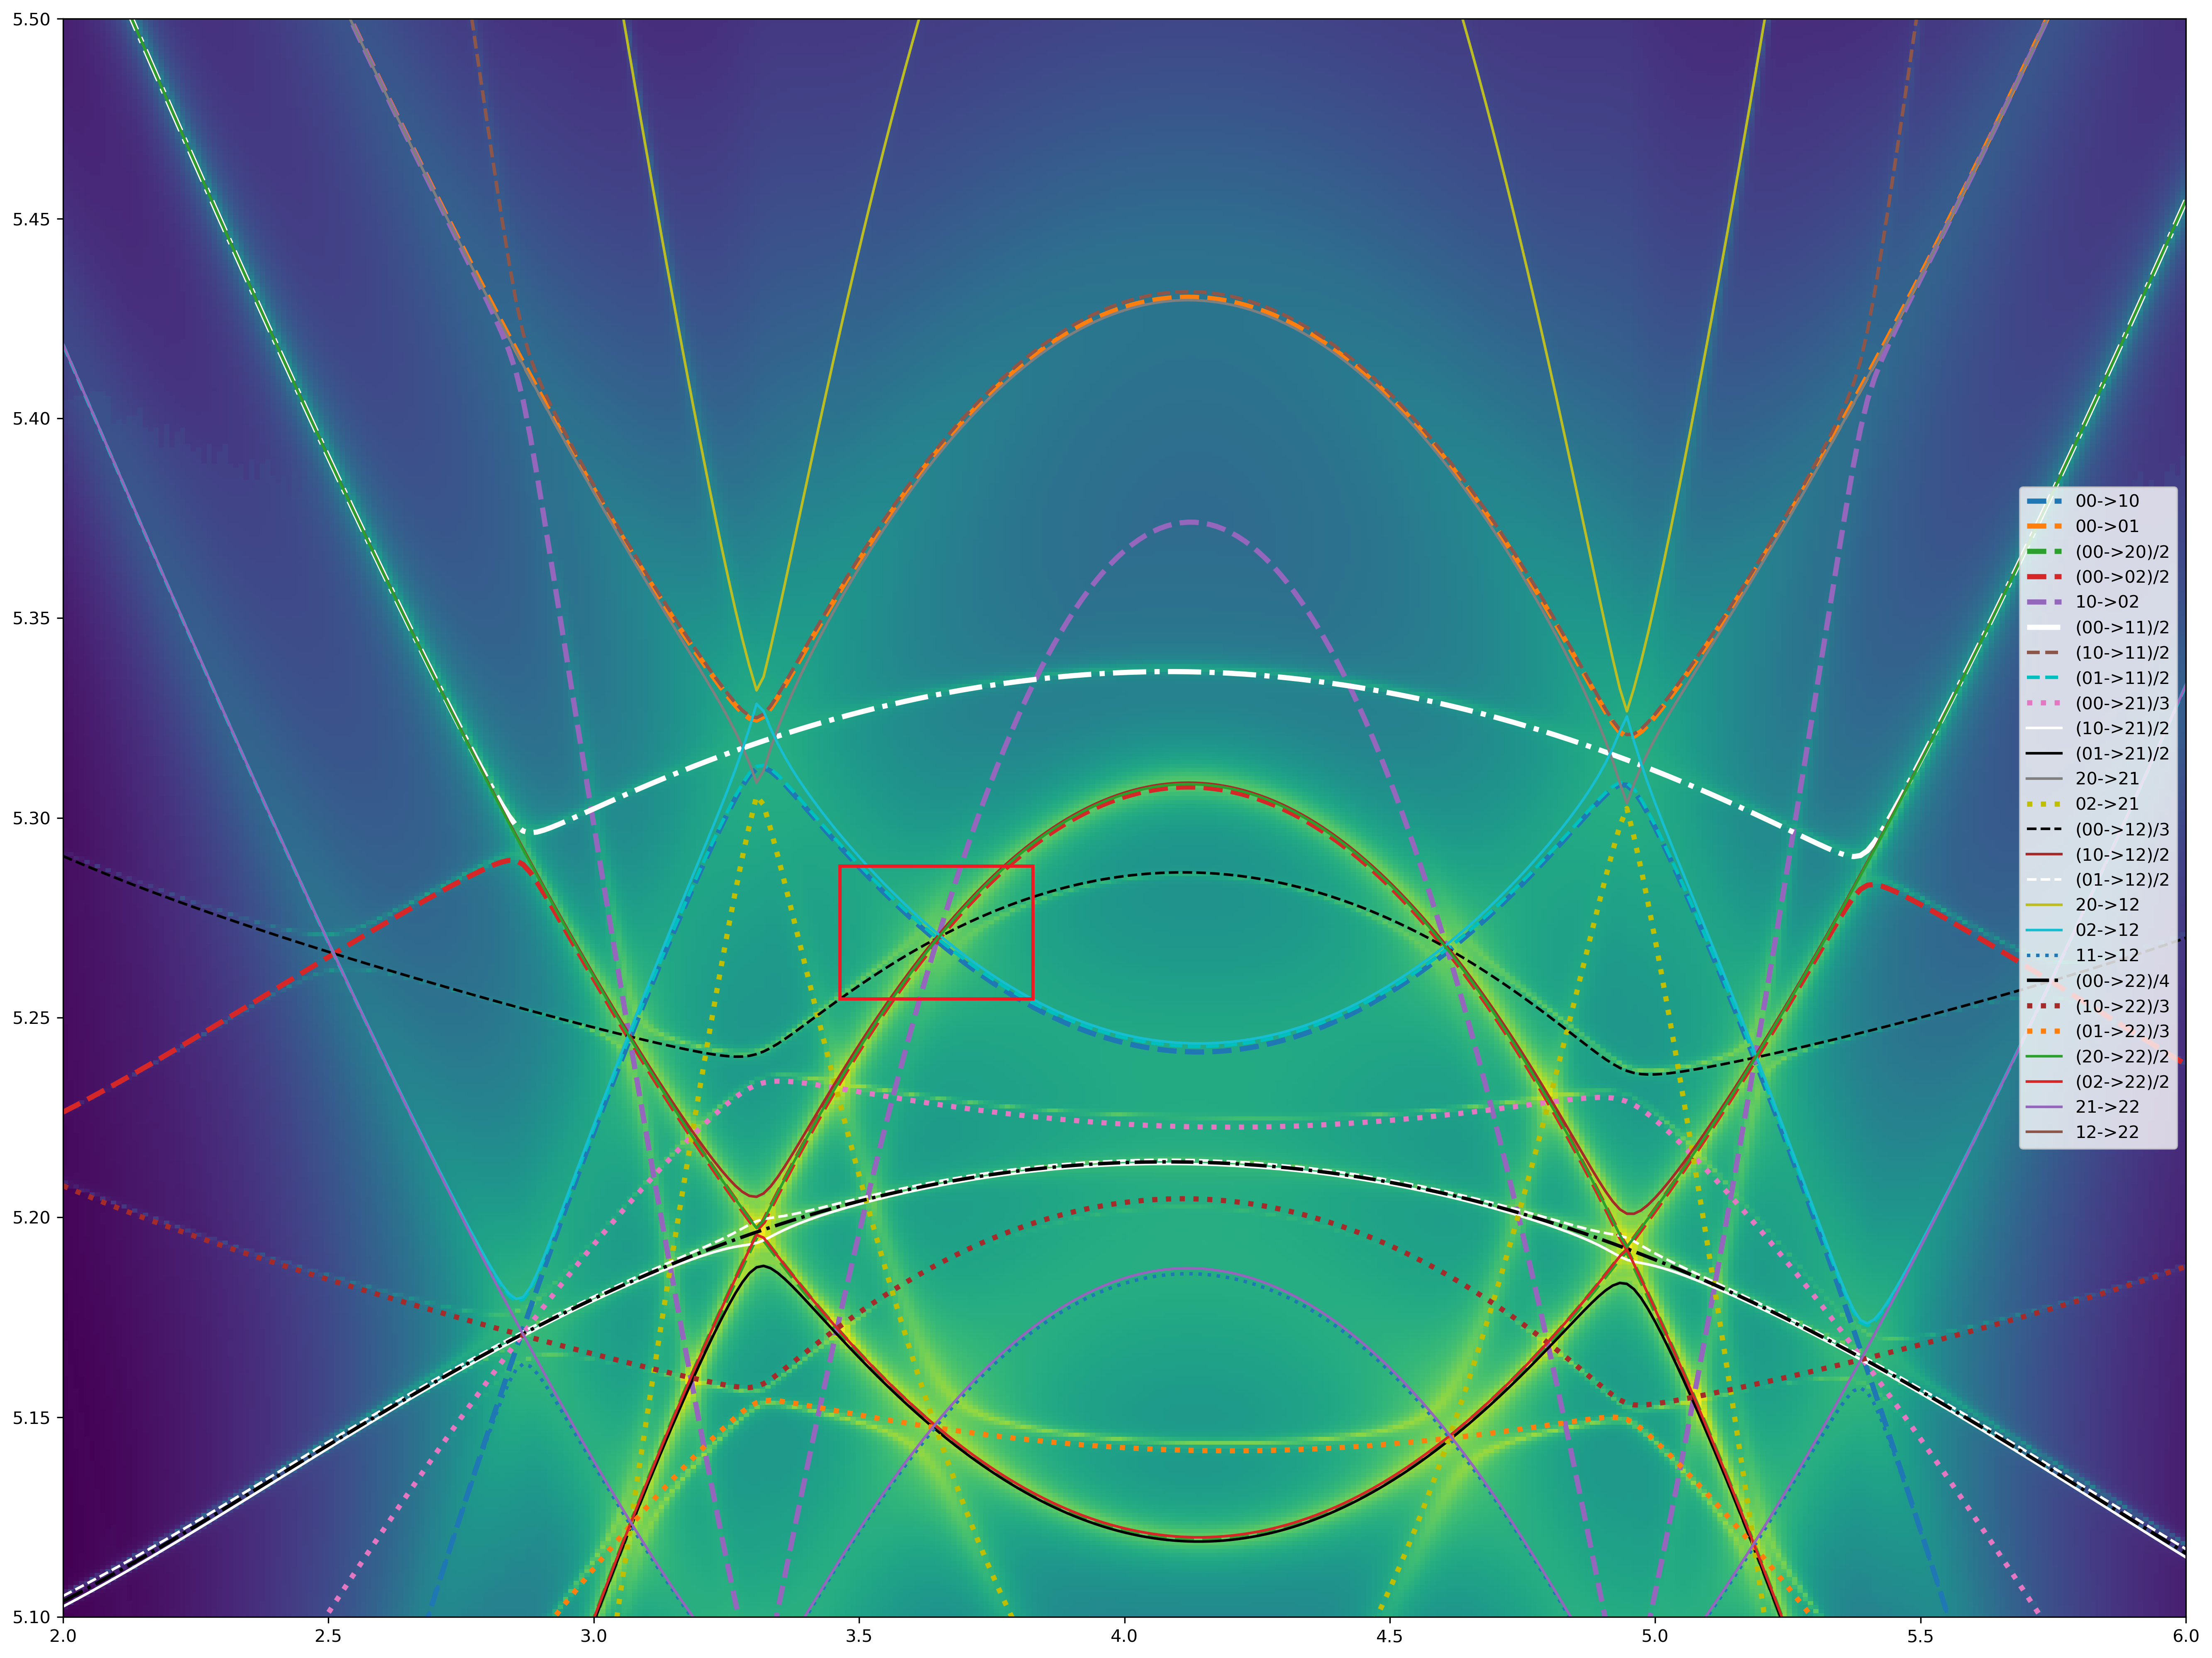
\includegraphics[width=\linewidth]{spectr}
	\caption{Two-tone spectroscopy with transitions lines. In the red frame, four transitions intersect, three of which originate from the state $\ket{00}$ to $\ket{10}$, two-photon
		$\ket{02}$, three-photon
		$\ket{12}$ and the fourth from  $\ket{10}$ to  $\ket{02}$, where $\ket{ij}$ denote the $ij-th$ energy eigenstate of the transmon system, i,j represent first and second qubit respectively}
	\label{fig:spectr}
\end{figure}


 Let's described the anti-crossing highlighted in red in the picture. 
 
 

\bibliography{papers_bibliography}% Produces the bibliography via BibTeX.	
\end{document}